
% Diapositiva 1: Introducción a MediaPipe
\begin{frame}{¿Qué es MediaPipe?}
    \begin{itemize}
        \item Es una biblioteca de código abierto de Google para procesamiento de señales en tiempo real.
        \item Permite la implementación eficiente de modelos de Machine Learning en dispositivos móviles y de escritorio.
        \item Soporta múltiples plataformas como Android, iOS, y Python.
    \end{itemize}
\end{frame}

% Diapositiva 3: Soluciones preentrenadas
\begin{frame}{Soluciones preentrenadas}
    \begin{itemize}
        \item \textbf{Detección de pose:} Identificación de puntos clave en el cuerpo humano para análisis de movimiento.
        \item \textbf{Detección facial:} Seguimiento de rasgos faciales para aplicaciones como realidad aumentada y reconocimiento facial.
        \item \textbf{Detección de manos:} Segmentación y seguimiento de manos en tiempo real para gestos y control por movimientos.
    \end{itemize}
    \begin{center}
        \includegraphics[width=0.6\linewidth]{mediapipe_solutions.png}
    \end{center}
\end{frame}

% Diapositiva 3: Flujo de funcionamiento
\begin{frame}{Flujo de funcionamiento}
    \begin{enumerate}
        \item Captura de datos desde una cámara o archivo.
        \item Procesamiento mediante el gráfico de MediaPipe.
        \item Obtención de resultados como coordenadas de puntos clave o segmentación.
    \end{enumerate}
    \begin{center}
        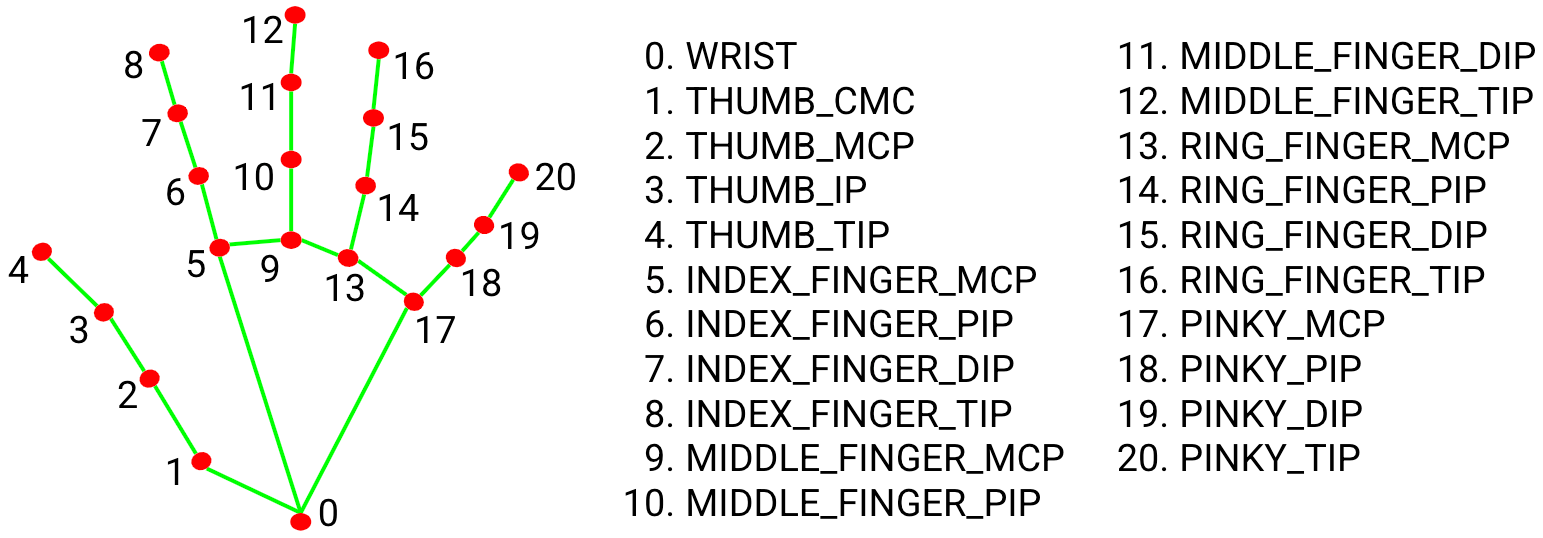
\includegraphics[width=0.6\linewidth]{01_MediaPipe/hand_landmarks.png}
    \end{center}
\end{frame}

% Diapositiva 4: Flujo de funcionamiento
\begin{frame}{Flujo de funcionamiento}
    \begin{enumerate}
        \item Captura de datos desde una cámara o archivo.
        \item Procesamiento mediante el gráfico de MediaPipe.
        \item Obtención de resultados como coordenadas de puntos clave o segmentación.
    \end{enumerate}
    \begin{center}
        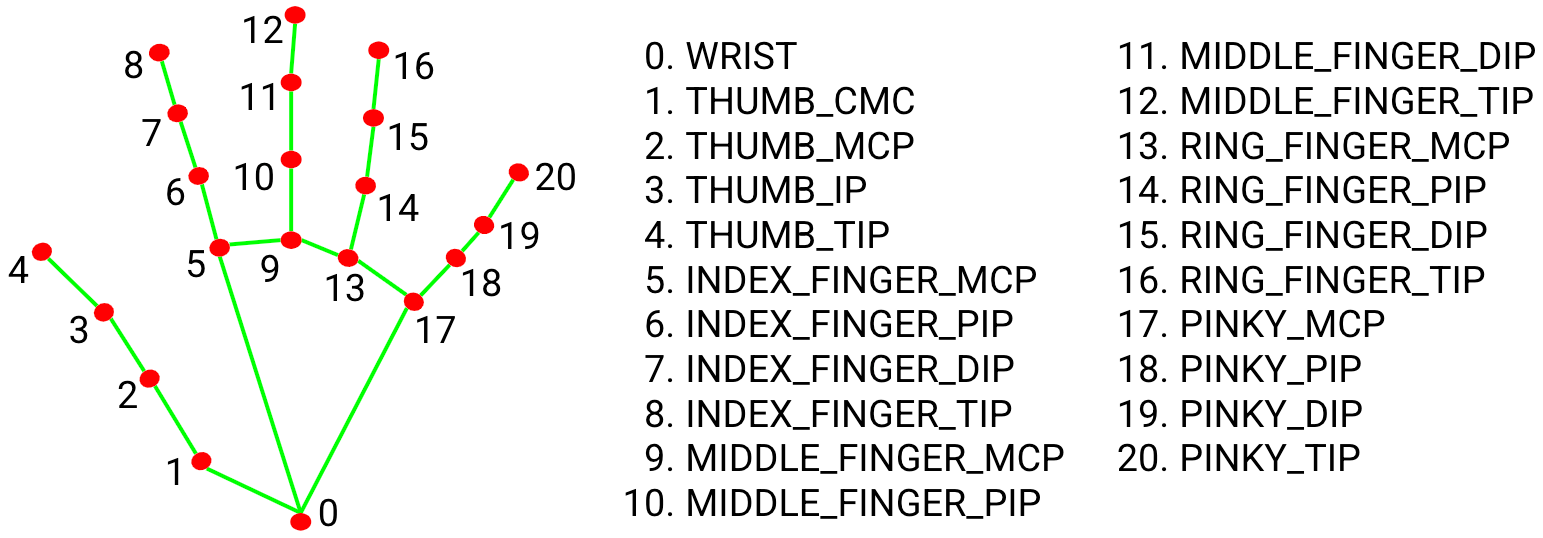
\includegraphics[width=0.6\linewidth]{01_MediaPipe/hand_landmarks.png}
    \end{center}
\end{frame}

